\section{Вычислительный эксперимент} \label{section:experiments}

    В этом разделе представлены результаты экспериментов по применению аппроксимации нулевого порядка \texttt{JAGUAR} к различным задачам оптимизации <<черного ящика>>. Результаты включают детерминированный и стохастический случаи алгоритма Франка-Вульфа.
    
\subsection{Постановка эксперимента}

    Рассматривается модель логистической регрессии на множестве $Q$ вида:
    \begin{align*}
        \min_{w \in Q} \left\{ f(w) = \frac{1}{m} \sum_{k = 1}^{m} \log \left( 1 + \exp \left[ -y_k (Xw)_k \right] \right) + \frac{1}{2C} \| w \|^2 \right\}.
    \end{align*}

    Также рассматривается модель SVM на множестве $Q$ вида:
    \begin{align*}
        \min_{w \in Q, b \in \mathbb{R}} \left\{ f(w, b) = \frac{1}{m} \sum_{k = 1}^{m} \left( 1 - y_k [(Xw)_k - b] \right)_+ + \frac{1}{2C} \| w \|^2 \right\}.
    \end{align*}

    В обеих задачах используется регуляризационный член $C = 10$. В качестве минимизирующего множества $Q$ рассматриваются симплекс $\Delta_d$ и $l_2$-шар. Для решения задачи классификации используются классические датасеты MNIST \cite{deng2012mnist} и Mushrooms \cite{chang2011libsvm}.
    
    В эксперименте сравниваются различные методы аппроксимации. В качестве базовых оценок градиентов рассматриваются $l_2$-\textit{сглаживание} \eqref{eq:l2_approx} и \textit{полная аппроксимация} \eqref{eq:full_approx}. Показывается, что алгоритм, использующий аппроксимацию \texttt{JAGUAR} (алгоритмы \ref{alg:JAGUAR_nonstoch} и \ref{alg:FW_stoch}), работает лучше всего.

\subsection{Детерминированный алгоритм Франка-Вульфа}
    
    В этом разделе рассматриваем детерминированный шум вида $f_\delta(x) = \text{round}(f(x), 5)$, т.е. округление значения функции $f$ до пятого знака после запятой. На рисунке \ref{fig:FW_determ} показана сходимость детерминированного алгоритма Франка-Вульфа с аппроксимацией нулевого порядка. У алгоритм Франка-Вульфа с \texttt{JAGUAR} (алгоритм \ref{alg:FW}) результаты лучше, чем у базовых алгоритмов. Это наблюдение подтверждает теоретические выводы. 
    
    \begin{figure}[H]
        \centering
        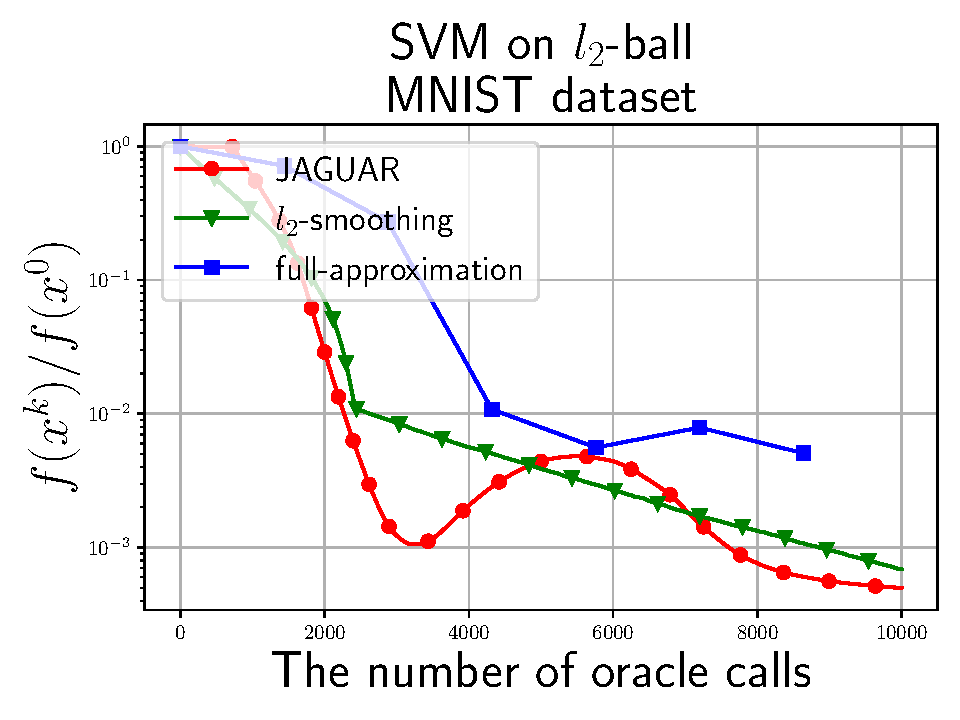
\includegraphics[width=0.49\textwidth]{figures/None_stochastics_FW_SVM_L2_MNIST.pdf}
        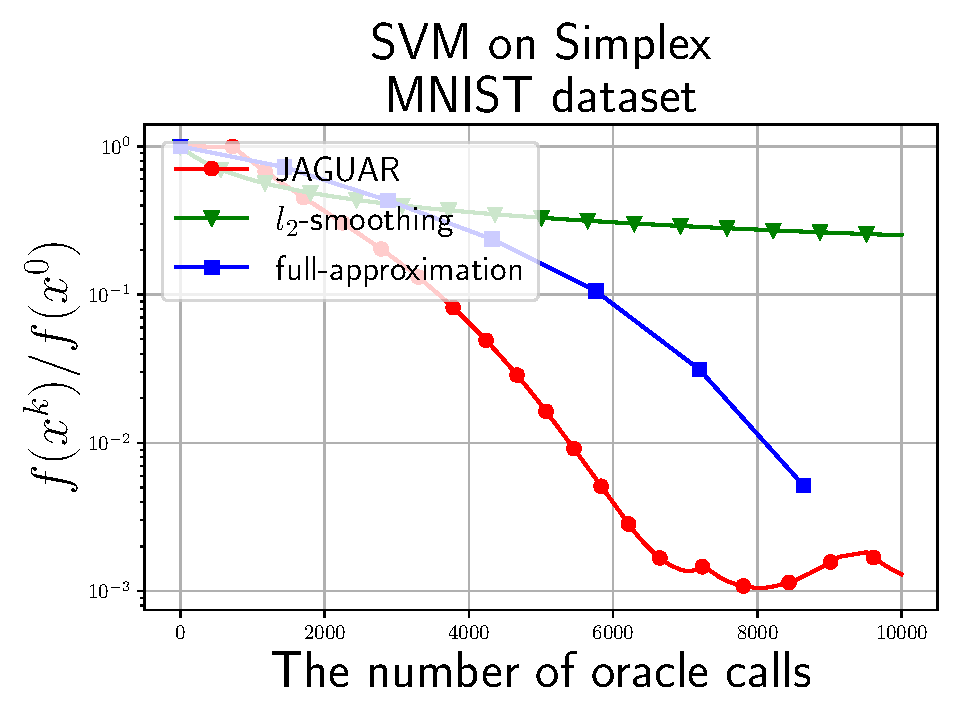
\includegraphics[width=0.49\textwidth]{figures/None_stochastics_FW_SVM_Simplex_MNIST.pdf}

        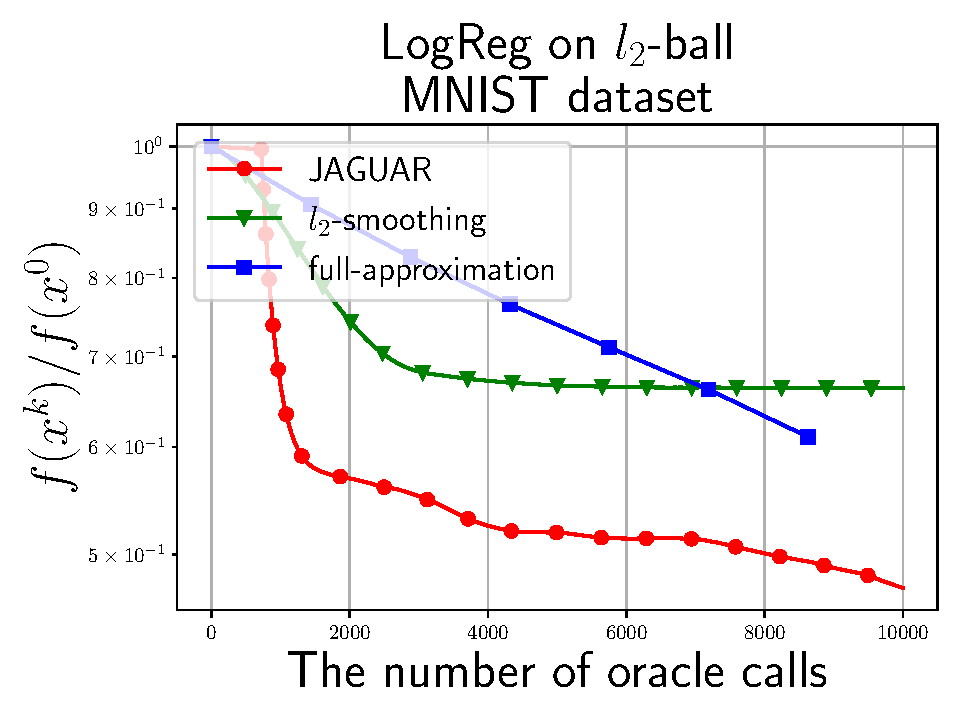
\includegraphics[width=0.49\textwidth]{figures/None_stochastics_FW_LogReg_L2_MNIST.pdf}
        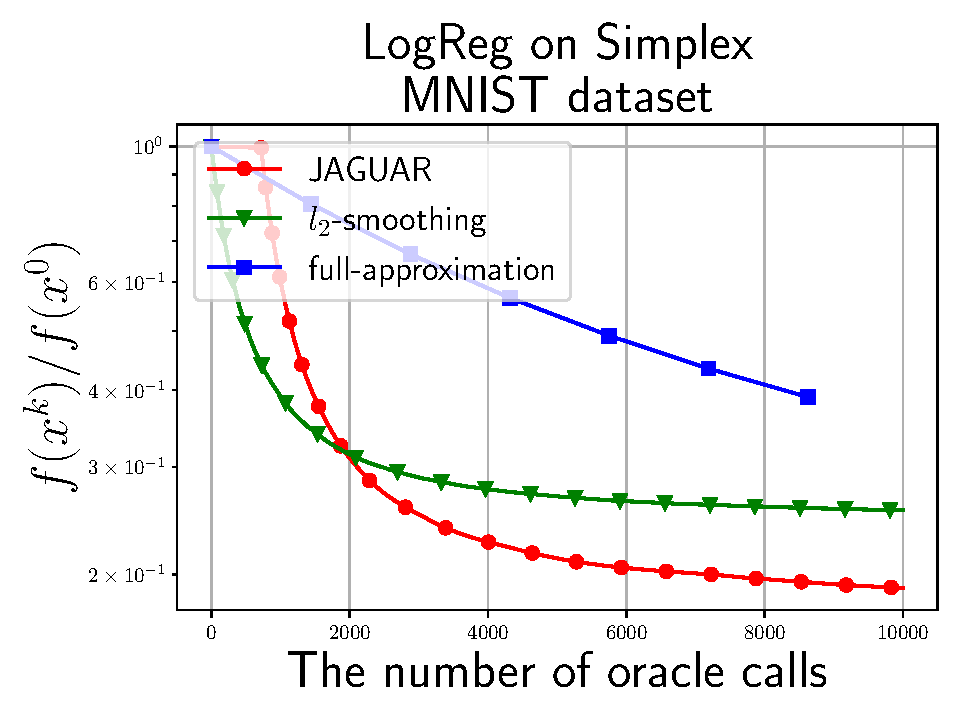
\includegraphics[width=0.49\textwidth]{figures/None_stochastics_FW_LogReg_Simplex_MNIST.pdf}
        
        \caption{Детерминированный алгоритм Франка-Вульфа.}
        \label{fig:FW_determ}
    \end{figure}

\subsection{Стохастический алгоритм Франка-Вульфа}

    В этом разделе рассматривается стохастический шум вида $f_\delta(x, \xi) = f(x) + \xi; \xi \sim \mathcal{N}(0, 0.1)$. На рисунке \ref{fig:FW_stoch} показана сходимость стохастического алгоритма Франка-Вульфа с аппроксимацией нулевого порядка. Теоретические выводы подтверждаются наблюдениями. Алгоритм Франка-Вульфа с \texttt{JAGUAR} (алгоритм \ref{alg:FW_stoch}) устойчив к шуму и превосходит базовые алгоритмы.

    \begin{figure}[H]
        \centering
        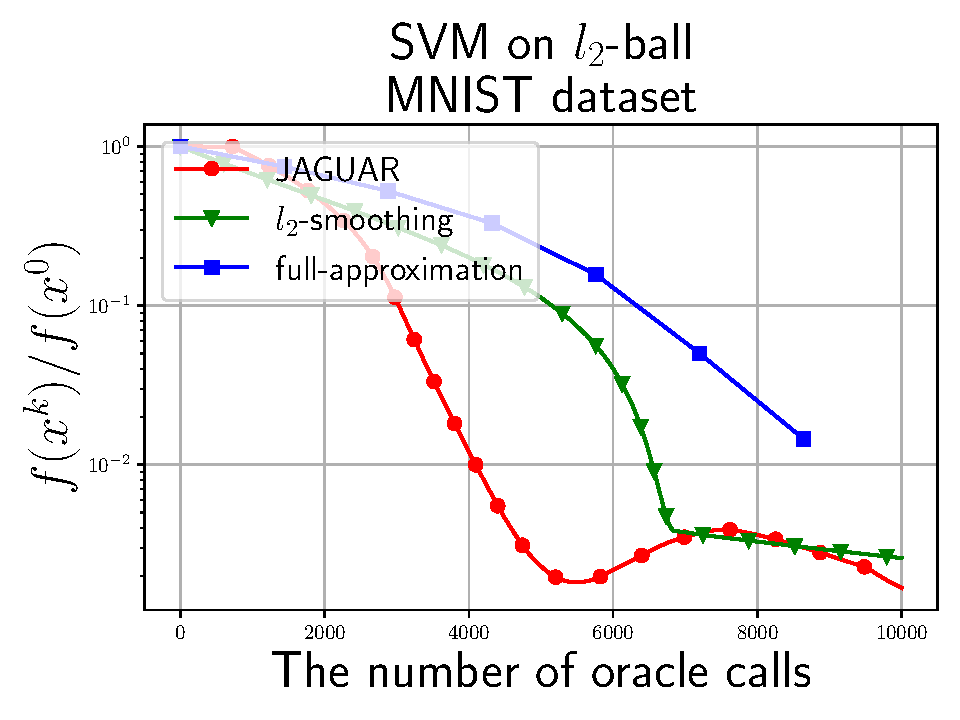
\includegraphics[width=0.49\textwidth]{figures/Stochastics_TPF_FW_SVM_L2_MNIST.pdf}
        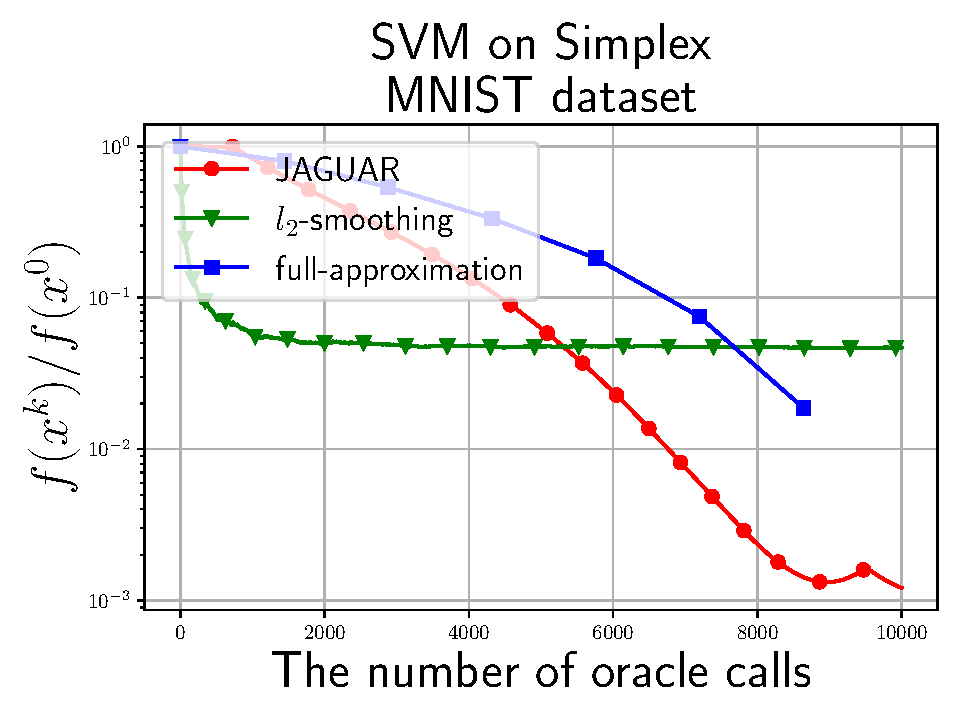
\includegraphics[width=0.49\textwidth]{figures/Stochastics_TPF_FW_SVM_Simplex_MNIST.pdf}

        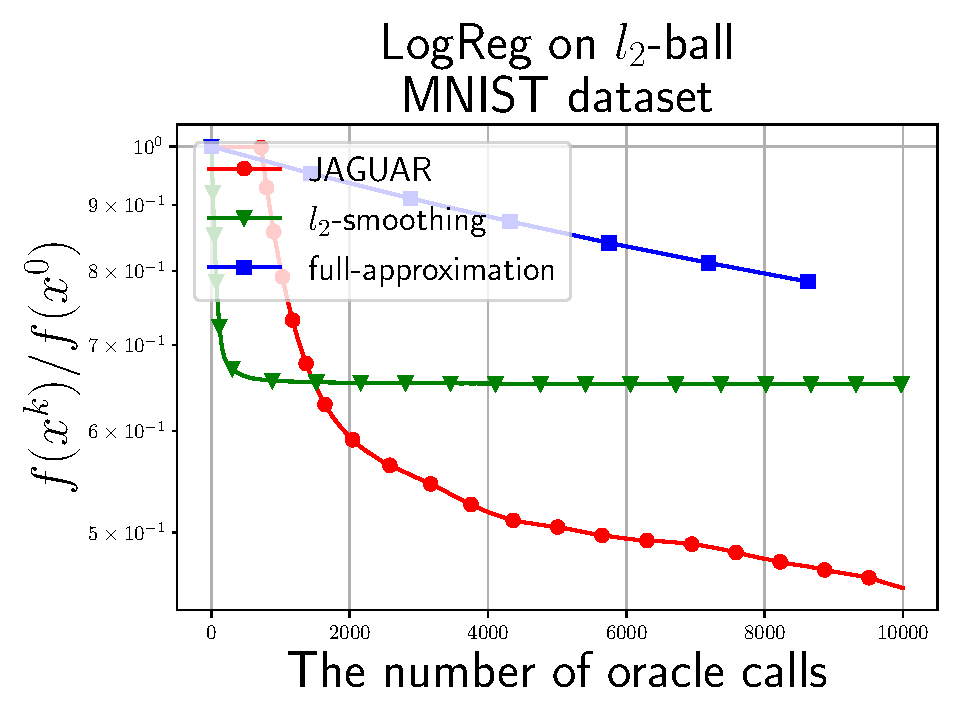
\includegraphics[width=0.49\textwidth]{figures/Stochastics_TPF_FW_LogReg_L2_MNIST.pdf}
        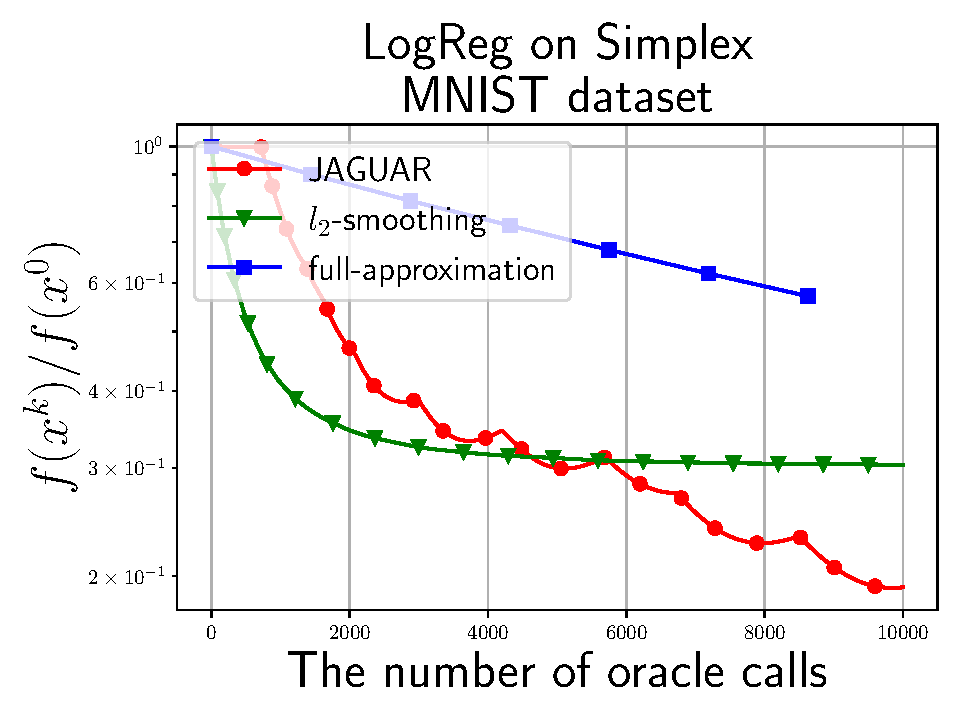
\includegraphics[width=0.49\textwidth]{figures/Stochastics_TPF_FW_LogReg_Simplex_MNIST.pdf}
        
        \caption{Стохастический алгоритм Франка-Вульфа.}
        \label{fig:FW_stoch}
    \end{figure}